\documentclass{article}

% Required packages
\usepackage{amssymb}
\usepackage{amsmath}
\usepackage{graphicx}
\usepackage{geometry}
\usepackage{tikz}
\usepackage{array}
\usepackage{booktabs}
\usepackage{enumitem}
\usepackage{listings}
\usepackage{xcolor}
\usepackage{fancyhdr}
\usepackage{float}
\usepackage{subcaption}
\usepackage{comment}

% Set page geometry
\geometry{a4paper, margin=1in}

% Configure listings for Python
\lstset{
  language=Python,
  basicstyle=\ttfamily\footnotesize,
  numbers=left,
  numberstyle=\tiny\color{gray},
  frame=single,
  breaklines=true,
  breakatwhitespace=true,
  captionpos=b,
  tabsize=4,
  showspaces=false,
  showstringspaces=false,
  showtabs=false,
  commentstyle=\color{gray}\textit,
  keywordstyle=\color{blue}\bfseries,
  stringstyle=\color{red}
}

\begin{document}

\pagestyle{fancy}
\chead{DSC 255: Machine Learning Fundamentals (Spring 2025)}
\lhead{Homework 10}
\rhead{Randall Rogers}

%------------------
% Solution for (a)
%------------------
\subsection*{Solution 1}
\noindent\rule{\textwidth}{0.4pt}\\

\subsubsection*{Step 1: Identify the network architecture}
\parbox{\textwidth}{
We are given the following about a feedforward neural net:
\begin{itemize}
    \item Input layer ($L_i$): 10 nodes
    \item Hidden layer 1 ($L_{hl1}$): 1000 nodes
    \item Hidden layer 2 ($L_{hl2}$): 1000 nodes
    \item Hidden layer 3 ($L_{hl3}$): 1000 nodes
    \item Hidden layer 4 ($L_{hl4}$): 1000 nodes
    \item Output layer ($L_o$): 1 node
\end{itemize}

}

\subsubsection*{Step 2: Calculate parameters between each layer pair}
\parbox{\textwidth}{
In a fully connected neural network, the number of parameters between two adjacent layers is the product of the number of nodes plus an offset term at each node.
Since, we are only looking for the approximate number of parameters, we can ignore the offset terms and the number of parametersis the following:
\begin{center}
  \begin{align*}
    \text{number of parameters} &\approx (L_i \cdot L_{hl1}) + (L_{hl1} \cdot L_{hl2}) + (L_{hl2} \cdot L_{hl3}) + (L_{hl3} \cdot L_{hl4}) + (L_{hl4} \cdot L_o)\\
    \text{number of parameters} &\approx (10 \cdot 1000) + (1000 \cdot 1000) + (1000 \cdot 1000) + (1000 \cdot 1)\\
    \text{number of parameters} &\approx 10,000 + 1,000,000 + 1,000,000 + 1,000,000 + 1,000\\
    \text{number of parameters} &\approx 3,011,000
  \end{align*}
\end{center}
}

\subsubsection*{\normalfont}{$\therefore$ The neural network has approximately 3,011,000 parameters.}

\noindent\rule{\textwidth}{0.4pt}\\

\newpage

\subsection*{Solution 2}
\noindent\rule{\textwidth}{0.4pt}\\

\subsubsection*{Step 1: Define probability of label using softmax}
\parbox{\textwidth}{
The probability of a label $j$ using softmax is defined as:

$$Pr(y_i) = \frac{e^{y_i}}{\sum_{j=1}^{n} e^{y_j}}$$

}

\subsubsection*{Step 2: Calculate probabilities}
\parbox{\textwidth}{
Now we can calculate the softmax probability for each label:
\begin{align*}
Pr(y_1) &= \frac{e^{y_1}}{\sum_{j=1}^{4} e^{y_j}} = \frac{e^{y_1}}{e^{y_1}+e^{y_2}+e^{y_3}+e^{y_4}} = \frac{e^{1.0}}{5.0862} \approx \frac{2.7183}{5.0862} \approx 0.5344\\
Pr(y_2) &= \frac{e^{y_2}}{\sum_{j=1}^{4} e^{y_j}} = \frac{e^{y_1}}{e^{y_1}+e^{y_2}+e^{y_3}+e^{y_4}} = \frac{e^{0.0}}{5.0862} = \frac{1.0000}{5.0862} \approx 0.1966\\
Pr(y_3) &= \frac{e^{y_3}}{\sum_{j=1}^{4} e^{y_j}} = \frac{e^{y_1}}{e^{y_1}+e^{y_2}+e^{y_3}+e^{y_4}} = \frac{e^{-1.0}}{5.0862} \approx \frac{0.3679}{5.0862} \approx 0.0723\\
Pr(y_4) &= \frac{e^{y_4}}{\sum_{j=1}^{4} e^{y_j}} = \frac{e^{y_1}}{e^{y_1}+e^{y_2}+e^{y_3}+e^{y_4}} = \frac{e^{0.0}}{5.0862} = \frac{1.0000}{5.0862} \approx 0.1966
\end{align*}
}

\subsubsection*{Step 3: Identify the most likely label}
\parbox{\textwidth}{
Comparing the probabilities:
\begin{align*}
Pr(y_1) &\approx 0.5344\\
Pr(y_2) &\approx 0.1966\\
Pr(y_3) &\approx 0.0723\\
Pr(y_4) &\approx 0.1966
\end{align*}

Hence, $P(y_1)$ has the highest probability.
}

\subsubsection*{\normalfont}{$\therefore$ The most likely label is label 1 ($y_1$), with a probability of approximately 0.5344 (or about 53.44\%).}

\noindent\rule{\textwidth}{0.4pt}\\

\newpage

\subsection*{Solution 3}
\noindent\rule{\textwidth}{0.4pt}\\


\subsubsection*{Step 1: Neural Network architecture}
\parbox{\textwidth}{
The neural network has the following properties:
\begin{itemize}
    \item 2 input units: $x_1$ and $x_2$
    \item 2 hidden units with ReLU activation
    \item 1 output unit
\end{itemize}

Where the ReLU (Rectified Linear Unit) activation function is defined as:

$$\text{ReLU}(z) = \max(0, z)$$

}

\subsubsection*{Step 2: Define structure}
\parbox{\textwidth}{
Let:
\begin{itemize}
    \item $h_1$ and $h_2$ as the outputs of the two hidden units
    \item $W^{(1)}$ as the weight matrix from input to hidden layer
    \item $b^{(1)}$ as the bias vector for the hidden layer
    \item $W^{(2)}$ as the weight vector from hidden to output layer
    \item $b^{(2)}$ as the bias for the output unit
\end{itemize}

The forward pass through the network can be written as:
\begin{align*}
h_1 &= \text{ReLU}(w_{11}^{(1)}x_1 + w_{12}^{(1)}x_2 + b_1^{(1)})\\
h_2 &= \text{ReLU}(w_{21}^{(1)}x_1 + w_{22}^{(1)}x_2 + b_2^{(1)})\\
y &= w_{1}^{(2)}h_1 + w_{2}^{(2)}h_2 + b^{(2)}
\end{align*}

We need to find values for these weights and biases such that the output $y$ matches the XOR function.
}

\subsubsection*{Step 3: Determine the weights and biases}
\parbox{\textwidth}{
The hidden units should have the following logic:
\begin{itemize}
    \item $h_1$ should activate (output positive value) when at least one input is 1
    \item $h_2$ should activate (output positive value) when both inputs are 1
\end{itemize}

For $h_1$, we want:
\begin{align*}
h_1(0,0) &= \text{ReLU}(w_{11}^{(1)} \cdot 0 + w_{12}^{(1)} \cdot 0 + b_1^{(1)}) = 0\\
h_1(0,1) &= \text{ReLU}(w_{11}^{(1)} \cdot 0 + w_{12}^{(1)} \cdot 1 + b_1^{(1)}) > 0\\
h_1(1,0) &= \text{ReLU}(w_{11}^{(1)} \cdot 1 + w_{12}^{(1)} \cdot 0 + b_1^{(1)}) > 0\\
h_1(1,1) &= \text{ReLU}(w_{11}^{(1)} \cdot 1 + w_{12}^{(1)} \cdot 1 + b_1^{(1)}) > 0
\end{align*}

Let $w_{11}^{(1)} = 1$, $w_{12}^{(1)} = 1$, and $b_1^{(1)} = -0.5$, then subsitiute into equations above to see if conditions are met:
\begin{align*}
h_1(0,0) &= \text{ReLU}(0 + 0 - 0.5) = \text{ReLU}(-0.5) = 0\\
h_1(0,1) &= \text{ReLU}(0 + 1 - 0.5) = \text{ReLU}(0.5) = 0.5\\
h_1(1,0) &= \text{ReLU}(1 + 0 - 0.5) = \text{ReLU}(0.5) = 0.5\\
h_1(1,1) &= \text{ReLU}(1 + 1 - 0.5) = \text{ReLU}(1.5) = 1.5
\end{align*}

We have: $h_1(0,0) = 0$, $h_1(1,0) = 0.5 > 0$, $h_1(0,1) = 0.5 > 0$, and $h_1(1,1) = 1.5 > 0$.
Hence, the conditions for $h_1$ are met.

For $h_2$, we want:
\begin{align*}
h_2(0,0) &= \text{ReLU}(w_{21}^{(1)} \cdot 0 + w_{22}^{(1)} \cdot 0 + b_2^{(1)}) = 0\\
h_2(0,1) &= \text{ReLU}(w_{21}^{(1)} \cdot 0 + w_{22}^{(1)} \cdot 1 + b_2^{(1)}) = 0\\
h_2(1,0) &= \text{ReLU}(w_{21}^{(1)} \cdot 1 + w_{22}^{(1)} \cdot 0 + b_2^{(1)}) = 0\\
h_2(1,1) &= \text{ReLU}(w_{21}^{(1)} \cdot 1 + w_{22}^{(1)} \cdot 1 + b_2^{(1)}) > 0
\end{align*}

Let, $w_{21}^{(1)} = 1$, $w_{22}^{(1)} = 1$, and $b_2^{(1)} = -1.5$, then subsitiute into equations above to see if conditions are met:
\begin{align*}
h_2(0,0) &= \text{ReLU}(0 + 0 - 1.5) = \text{ReLU}(-1.5) = 0\\
h_2(0,1) &= \text{ReLU}(0 + 1 - 1.5) = \text{ReLU}(-0.5) = 0\\
h_2(1,0) &= \text{ReLU}(1 + 0 - 1.5) = \text{ReLU}(-0.5) = 0\\
h_2(1,1) &= \text{ReLU}(1 + 1 - 1.5) = \text{ReLU}(0.5) = 0.5
\end{align*}
}

We have: $h_2(0,0) = 0$, $h_2(1,0) = 0$, $h_2(0,1) = 0$, and $h_2(1,1) = 0.5 > 0$.
Hence, the conditions for $h_2$ are met.

\subsubsection*{Step 5: Determine the output layer weights}
\parbox{\textwidth}{
The output $y$ is defined as:

$$y = w_{1}^{(2)}h_1 + w_{2}^{(2)}h_2 + b^{(2)}$$

We want:
\begin{align*}
y(0,0) &= w_{1}^{(2)} \cdot 0 + w_{2}^{(2)} \cdot 0 + b^{(2)} = 0\\
y(0,1) &= w_{1}^{(2)} \cdot 0.5 + w_{2}^{(2)} \cdot 0 + b^{(2)} = 1\\
y(1,0) &= w_{1}^{(2)} \cdot 0.5 + w_{2}^{(2)} \cdot 0 + b^{(2)} = 1\\
y(1,1) &= w_{1}^{(2)} \cdot 1.5 + w_{2}^{(2)} \cdot 0.5 + b^{(2)} = 0
\end{align*}

From the $y(0,0)$ equation, we get $b^{(2)} = 0$.
From the $y(0,1)$ and $y(1,0)$ equations, we get $w_{1}^{(2)} \cdot 0.5 = 1$, so $w_{1}^{(2)} = 2$.
From the $y(1,1)$ equation, we get $2 \cdot 1.5 + w_{2}^{(2)} \cdot 0.5 = 0$, which gives $3 + 0.5w_{2}^{(2)} = 0$, so $w_{2}^{(2)} = -6$.

Verify the weights and biases:
\begin{align*}
y(0,0) &= 2 \cdot 0 + (-6) \cdot 0 + 0 = 0 \\
y(0,1) &= 2 \cdot 0.5 + (-6) \cdot 0 + 0 = 1 \\
y(1,0) &= 2 \cdot 0.5 + (-6) \cdot 0 + 0 = 1 \\
y(1,1) &= 2 \cdot 1.5 + (-6) \cdot 0.5 + 0 = 3 - 3 = 0 
\end{align*}
}

\subsubsection*{\normalfont}{$\therefore$ the neural network implements the XOR function with the following parameters:}\\

\parbox{\textwidth}{

Input to hidden layer weights:\\

$$W^{(1)} = \begin{bmatrix} w_{11}^{(1)} & w_{12}^{(1)} \\ w_{21}^{(1)} & w_{22}^{(1)} \end{bmatrix} = \begin{bmatrix} 1 & 1 \\ 1 & 1 \end{bmatrix}$$

Hidden layer biases:\\
$$b^{(1)} = \begin{bmatrix} b_1^{(1)} \\ b_2^{(1)} \end{bmatrix} = \begin{bmatrix} -0.5 \\ -1.5 \end{bmatrix}$$

Hidden to output layer weights:\\
$$W^{(2)} = \begin{bmatrix} w_{1}^{(2)} & w_{2}^{(2)} \end{bmatrix} = \begin{bmatrix} 2 & -6 \end{bmatrix}$$

Output layer bias:\\
$$b^{(2)} = 0$$

}


\noindent\rule{\textwidth}{0.4pt}\\

\newpage

\subsection*{Solution 4 (a)}
\noindent\rule{\textwidth}{0.4pt}\\

\subsubsection*{Step 1}
\parbox{\textwidth}{

Let:
\begin{itemize}
    \item $h_{1}=\text{ReLU}(x_{1}+x_{2})$
    \item $h_{2}=\text{ReLU}(x_{1}+x_{2}-1)$
    \item $y=h_{1}-h_{2}$
\end{itemize}

Now, calculate $h_1$ and $h_2$ for each input combination:

For $(x_1, x_2) = (0, 0)$:

$$h_1 = \text{ReLU}(0 + 0) = \text{ReLU}(0) = 0 \hspace{0.25cm} \text{and} \hspace{0.25cm} h_2 = \text{ReLU}(0 + 0 - 1) = \text{ReLU}(-1) = 0$$

For $(x_1, x_2) = (0, 1)$:

$$h_1 = \text{ReLU}(0 + 1) = \text{ReLU}(1) = 1 \hspace{0.25cm} \text{and} \hspace{0.25cm} h_2 = \text{ReLU}(0 + 1 - 1) = \text{ReLU}(0) = 0$$

For $(x_1, x_2) = (1, 0)$:

$$h_1 = \text{ReLU}(1 + 0) = \text{ReLU}(1) = 1 \hspace{0.25cm} \text{and} \hspace{0.25cm} h_2 = \text{ReLU}(1 + 0 - 1) = \text{ReLU}(0) = 0$$


For $(x_1, x_2) = (1, 1)$:

$$h_1 = \text{ReLU}(1 + 1) = \text{ReLU}(2) = 2 \hspace{0.25cm} \text{and} \hspace{0.25cm} h_2 = \text{ReLU}(1 + 1 - 1) = \text{ReLU}(1) = 1$$

}

\subsubsection*{Step 2}
\parbox{\textwidth}{
Now we compute $y = h_1 - h_2$ for each case:

For $(x_1, x_2) = (0, 0)$: $y = h_1 - h_2 = 0 - 0 = 0$\\

For $(x_1, x_2) = (0, 1)$: $y = h_1 - h_2 = 1 - 0 = 1$\\

For $(x_1, x_2) = (1, 0)$: $y = h_1 - h_2 = 1 - 0 = 1$\\

For $(x_1, x_2) = (1, 1)$: $y = h_1 - h_2 = 2 - 1 = 1$

}

\subsubsection*{Step 3}
\parbox{\textwidth}{
Summarizing our results in a truth table:

\begin{center}
\begin{tabular}{|c|c|c|}
\hline
$x_1$ & $x_2$ & $y$ \\
\hline
0 & 0 & 0 \\
0 & 1 & 1 \\
1 & 0 & 1 \\
1 & 1 & 1 \\
\hline
\end{tabular}
\end{center}

This truth table corresponds to the logical OR function. The output is 1 when at least one of the inputs is 1, and 0 only when both inputs are 0.
}

\subsubsection*{\normalfont}{$\therefore$ The neural network realizes the OR function: $\text{OR}(x_1, x_2) = x_1 \vee x_2$.}

\noindent\rule{\textwidth}{0.4pt}\\

\newpage

\subsection*{Solution 4 (b)}
\noindent\rule{\textwidth}{0.4pt}\\

\subsubsection*{Step 1}
\parbox{\textwidth}{
Let:
\begin{itemize}
    \item $h_{1}=\text{ReLU}(x)$
    \item $h_{2}=\text{ReLU}(-x)$
    \item $y=h_{1}+h_{2}$
\end{itemize}

Determine behavior of each hidden unit for different values of $x \in \mathbb{R}$:

For $h_1 = \text{ReLU}(x)$:
\begin{align*}
h_1 = \begin{cases}
x & \text{if } x \geq 0 \\
0 & \text{if } x < 0
\end{cases}
\end{align*}

For $h_2 = \text{ReLU}(-x)$:
\begin{align*}
h_2 = \begin{cases}
-x & \text{if } x \leq 0 \\
0 & \text{if } x > 0
\end{cases}
\end{align*}

}

\subsubsection*{Step 2}
\parbox{\textwidth}{
Now we compute $y = h_1 + h_2$ by considering different cases:

Case 1: $x > 0$:
\begin{align*}
h_1 &= x \\
h_2 &= 0 \\
y &= h_1 + h_2 = x + 0 = x
\end{align*}

Case 2: $x < 0$:
\begin{align*}
h_1 &= 0 \\
h_2 &= -x \\
y &= h_1 + h_2 = 0 + (-x) = -x
\end{align*}

Case 3: $x = 0$:
\begin{align*}
h_1 &= \text{ReLU}(0) = 0 \\
h_2 &= \text{ReLU}(-0) = \text{ReLU}(0) = 0 \\
y &= h_1 + h_2 = 0 + 0 = 0
\end{align*}

Hence, we can write the output function as:
\begin{align*}
y = \begin{cases}
x & \text{if } x \geq 0 \\
-x & \text{if } x < 0
\end{cases}
\end{align*}
}

\subsubsection*{\normalfont}{$\therefore$ The neural network realizes the absolute value function: $f(x) = |x|$.}

\noindent\rule{\textwidth}{0.4pt}\\

\newpage

\subsection*{Solution 5}
\noindent\rule{\textwidth}{0.4pt}\\

\subsubsection*{Results Table}
\parbox{\textwidth}{
Below is a summary of the best models found for each dataset, including the value of $H$ (number of hidden units per layer), the number of iterations to convergence, and the final training error rate. For the noisy dataset, two hidden layers were used.

\begin{center}
\begin{tabular}{|c|c|c|c|}
\hline
\textbf{data} & \textbf{H value} & \textbf{iterations} & \textbf{error rate} \\
\hline
data1.txt & [fill] & [fill] & [fill] \\
data2.txt & [fill] & [fill] & [fill] \\
data3.txt & [fill] & [fill] & [fill] \\
data4.txt & [fill] & [fill] & [fill] \\
data5.txt & [fill] & [fill] & [fill] \\
noisy     & [fill] & [fill] & [fill] \\
\hline
\end{tabular}
\end{center}

Replace \texttt{[fill]} with the results from your Python runs.
}

\newpage

\subsection*{Solution 6}
\noindent\rule{\textwidth}{0.4pt}\\

\subsubsection*{Image Comparison: Orginal vs Normalized}
\parbox{\textwidth}{
  
Below is the image comparision.
\begin{figure}[H]
    \centering
    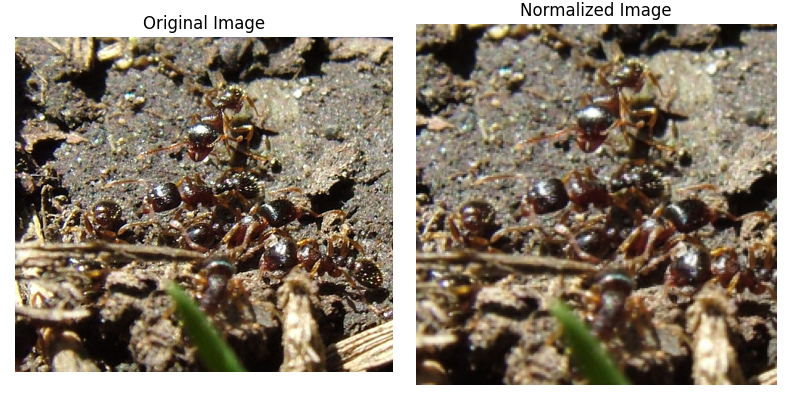
\includegraphics[width=0.7\textwidth]{q6_image_comparison.png}
    \caption{Left: Original image. Right: Normalized image that was resized and normalized for ResNet50 input.}
\end{figure}

}

\subsubsection*{Model Test Accuracies}
\parbox{\textwidth}{
\begin{center}
\begin{tabular}{|c|c|}
\hline
\textbf{classifier} & \textbf{test accuracy} \\
\hline
Logistic Regression & 0.9542 \\
k-NN ($k=1$) & 0.9673 \\
k-NN ($k=3$) & 0.9542 \\
k-NN ($k=5$) & 0.9608 \\
\hline
\end{tabular}
\end{center}
}

\noindent\rule{\textwidth}{0.4pt}\\

\newpage
\subsection*{Bonus: Evaluation}
\noindent\rule{\textwidth}{0.4pt}\\

\begin{figure}[h!] % [h!] tries to place the figure "here"
  \centering % Centers the image horizontally
  
\includegraphics[width=0.8\textwidth, height=0.45\textheight, keepaspectratio]{te_1.png}
  \caption{Hansin Evaluation}
  \label{fig:te1}
\end{figure}

\begin{figure}[h!]
  \centering
  
\includegraphics[width=0.8\textwidth, height=0.45\textheight, keepaspectratio]{te_2.png}
  \caption{Neo Evaluation}
  \label{fig:te2}
\end{figure}


\begin{comment}
  \begin{center} 
  \begin{tabular}{|c|c|c|} 
    \hline Stump Number (\%) & Training Accuracy (\%) \\ 
    \hline 
    1 & 16.32\\ 
    2 & 15.91 \\
    3 & 14.25 \\
    4 & 13.56 \\ 
    5 & 14.05  \\ 
    \hline
  \end{tabular}
\end{center}
\end{comment}

\begin{comment}
\subsection*{Solution 7}
\noindent\rule{\textwidth}{0.4pt}\\

\begin{figure}
  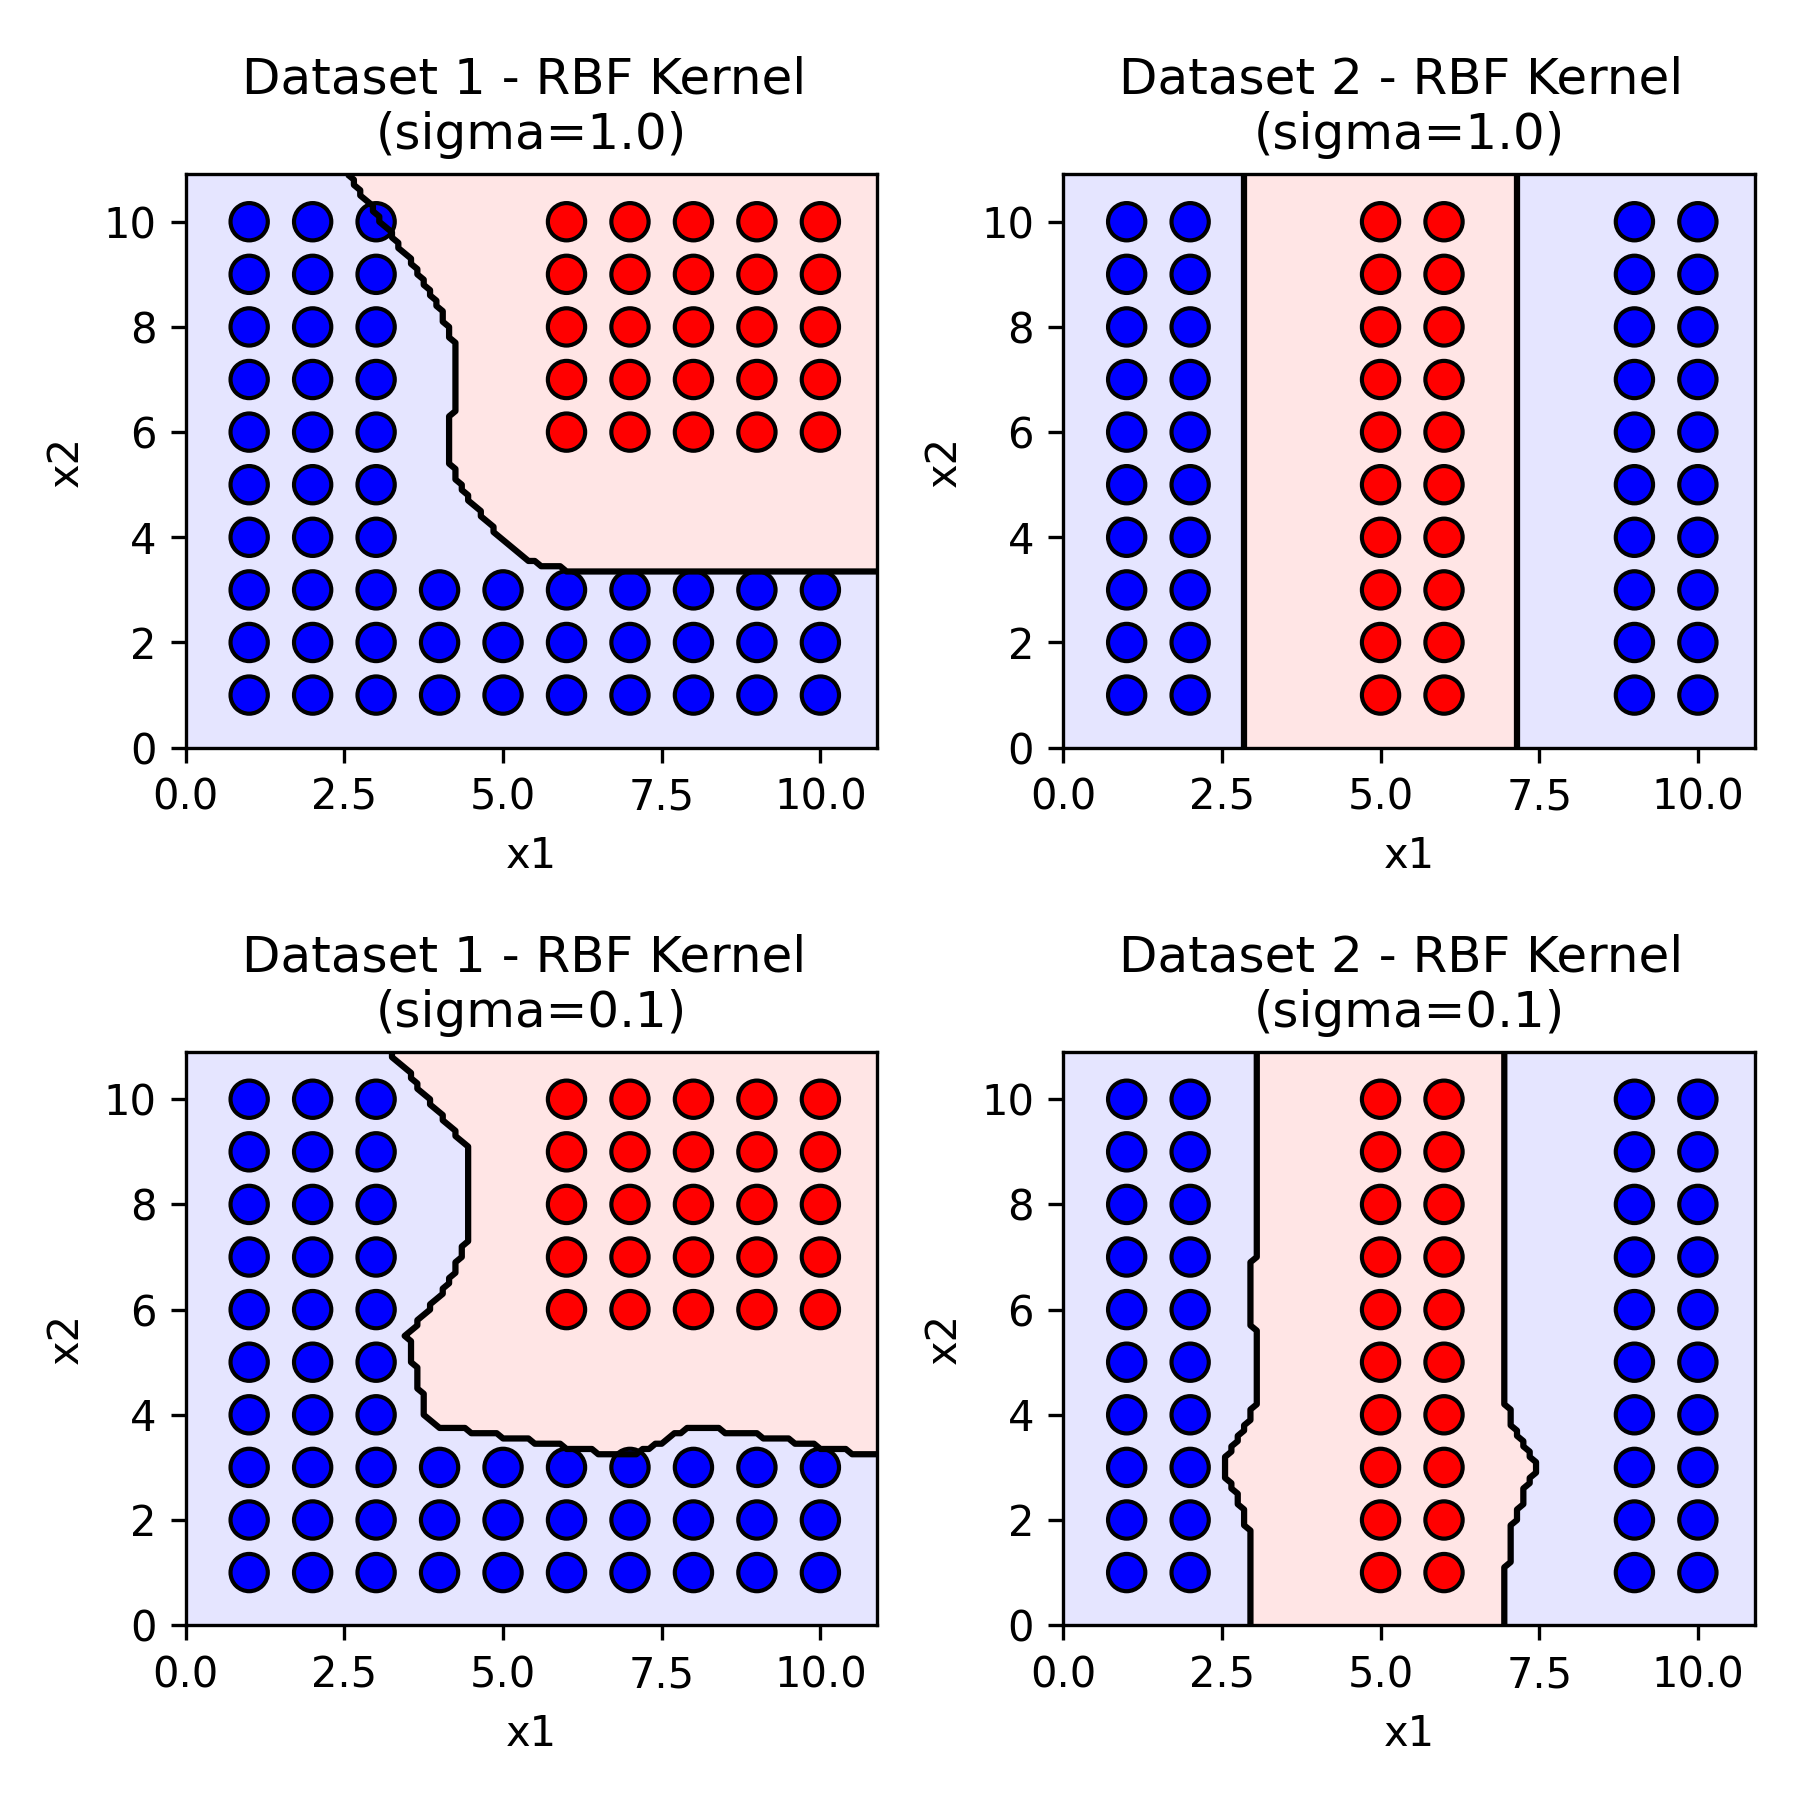
\includegraphics{part_b_rbf_kernel.png}
  \caption{Decision boundary for rbf kernel}
\end{figure}
\noindent\rule{\textwidth}{0.4pt}\\

\subsubsection*{Linear SVM}

\begin{center} 
  \begin{tabular}{|c|c|c|} 
    \hline C Value & Training Error (\%) & Test Error (\%) \\ 
    \hline 
    0.01 & 16.32 & 15.48\\ 
    0.1 & 15.91 & 16.36 \\
    1.0 & 14.25 & 14.04 \\
    10.0 & 13.56 & 13.16 \\ 
    100.0 & 14.05 & 14.78 \\ 
    \hline
  \end{tabular}
\end{center}
\parbox{\textwidth}{Based on the results above it seems that the data is linearly separable.}
\subsubsection*{Quadardic SVM}
\begin{center} 
  \begin{tabular}{|c|c|c|} 
    \hline Training Error (\%) & Test Error (\%)  & Support Vectors\\ 
    \hline 
    0.17 & 2.13 & 17906\\ 
    \hline
  \end{tabular}
\end{center}

\begin{lstlisting}
PYTHON CODE HERE
\end{lstlisting}
\end{comment}
\end{document}

